\documentclass[tikz,border=12pt]{standalone}

\begin{document}
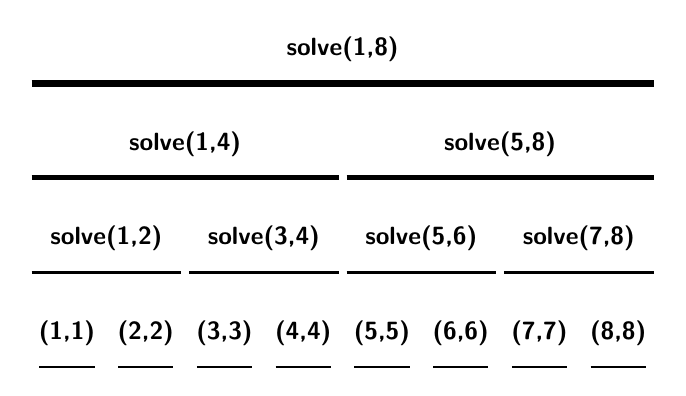
\begin{tikzpicture}[
    font=\small\sffamily\bfseries
]

\foreach \i in {1,...,8} {
    \draw[line width=0.8pt] (\i-0.35, 0) -- (\i+0.35, 0);
    \node[anchor=south] at (\i, 0.15) {(\i,\i)};
}

\foreach \i/\j in {1/2, 3/4, 5/6, 7/8} {
    \draw[line width=1.2pt] (\i-0.45, 1.2) -- (\j+0.45, 1.2);
}

\node[anchor=south] at (1.5, 1.35) {solve(1,2)};
\node[anchor=south] at (3.5, 1.35) {solve(3,4)};
\node[anchor=south] at (5.5, 1.35) {solve(5,6)};
\node[anchor=south] at (7.5, 1.35) {solve(7,8)};

\foreach \i/\j in {1/4, 5/8} {
    \draw[line width=1.8pt] (\i-0.45, 2.4) -- (\j+0.45, 2.4);
}

\node[anchor=south] at (2.5, 2.55) {solve(1,4)};
\node[anchor=south] at (6.5, 2.55) {solve(5,8)};

\draw[line width=2.8pt] (1-0.45, 3.6) -- (8+0.45, 3.6);
\node[anchor=south] at (4.5, 3.75) {solve(1,8)};

\end{tikzpicture}
\end{document}